\label{ch:supplementary_material}

\section*{Supplementary Material}
\beginsupplement

\begin{table}[htbp]
	\centering
	\caption{List of the focal species observed in the natural condition experiment within the Jena Experiment. Species had to flower in at least five plots with different frequency values to be considered as focal species.}
	\begin{tabular}{llllll}
		\toprule
		\textbf{Short} & \textbf{Name} & \textbf{German Name} & \textbf{Order} & \textbf{Family} & \textbf{Color} \\
		\midrule
		Ger   & \textit{Geranium pratense} & Wiesen-Storchschnabel & Geraniales & Geraniaceae & Purple \\
		Lat   & \textit{Lathyrus pratensis} & Wiesen-Platterbse & Fabales & Fabaceae & Yellow \\
		Lot   & \textit{Lotus corniculatus} & Gewöhnlicher Hornklee & Fabales & Fabaceae & Yellow \\
		Ono   & \textit{Onobrychis viciifolia} & Saat-Esparsette & Fabales & Fabaceae & Pink+White \\
		TP    & \textit{Trifolium pratense} & Wiesen-Klee & Fabales & Fabaceae & Purple \\
		\bottomrule
	\end{tabular}%
	\label{tab:Species}
\end{table}%

%%%%%%%%%%%%%%%%%%%%%%%%%%

\begin{figure} [H] %plot-design
\centering
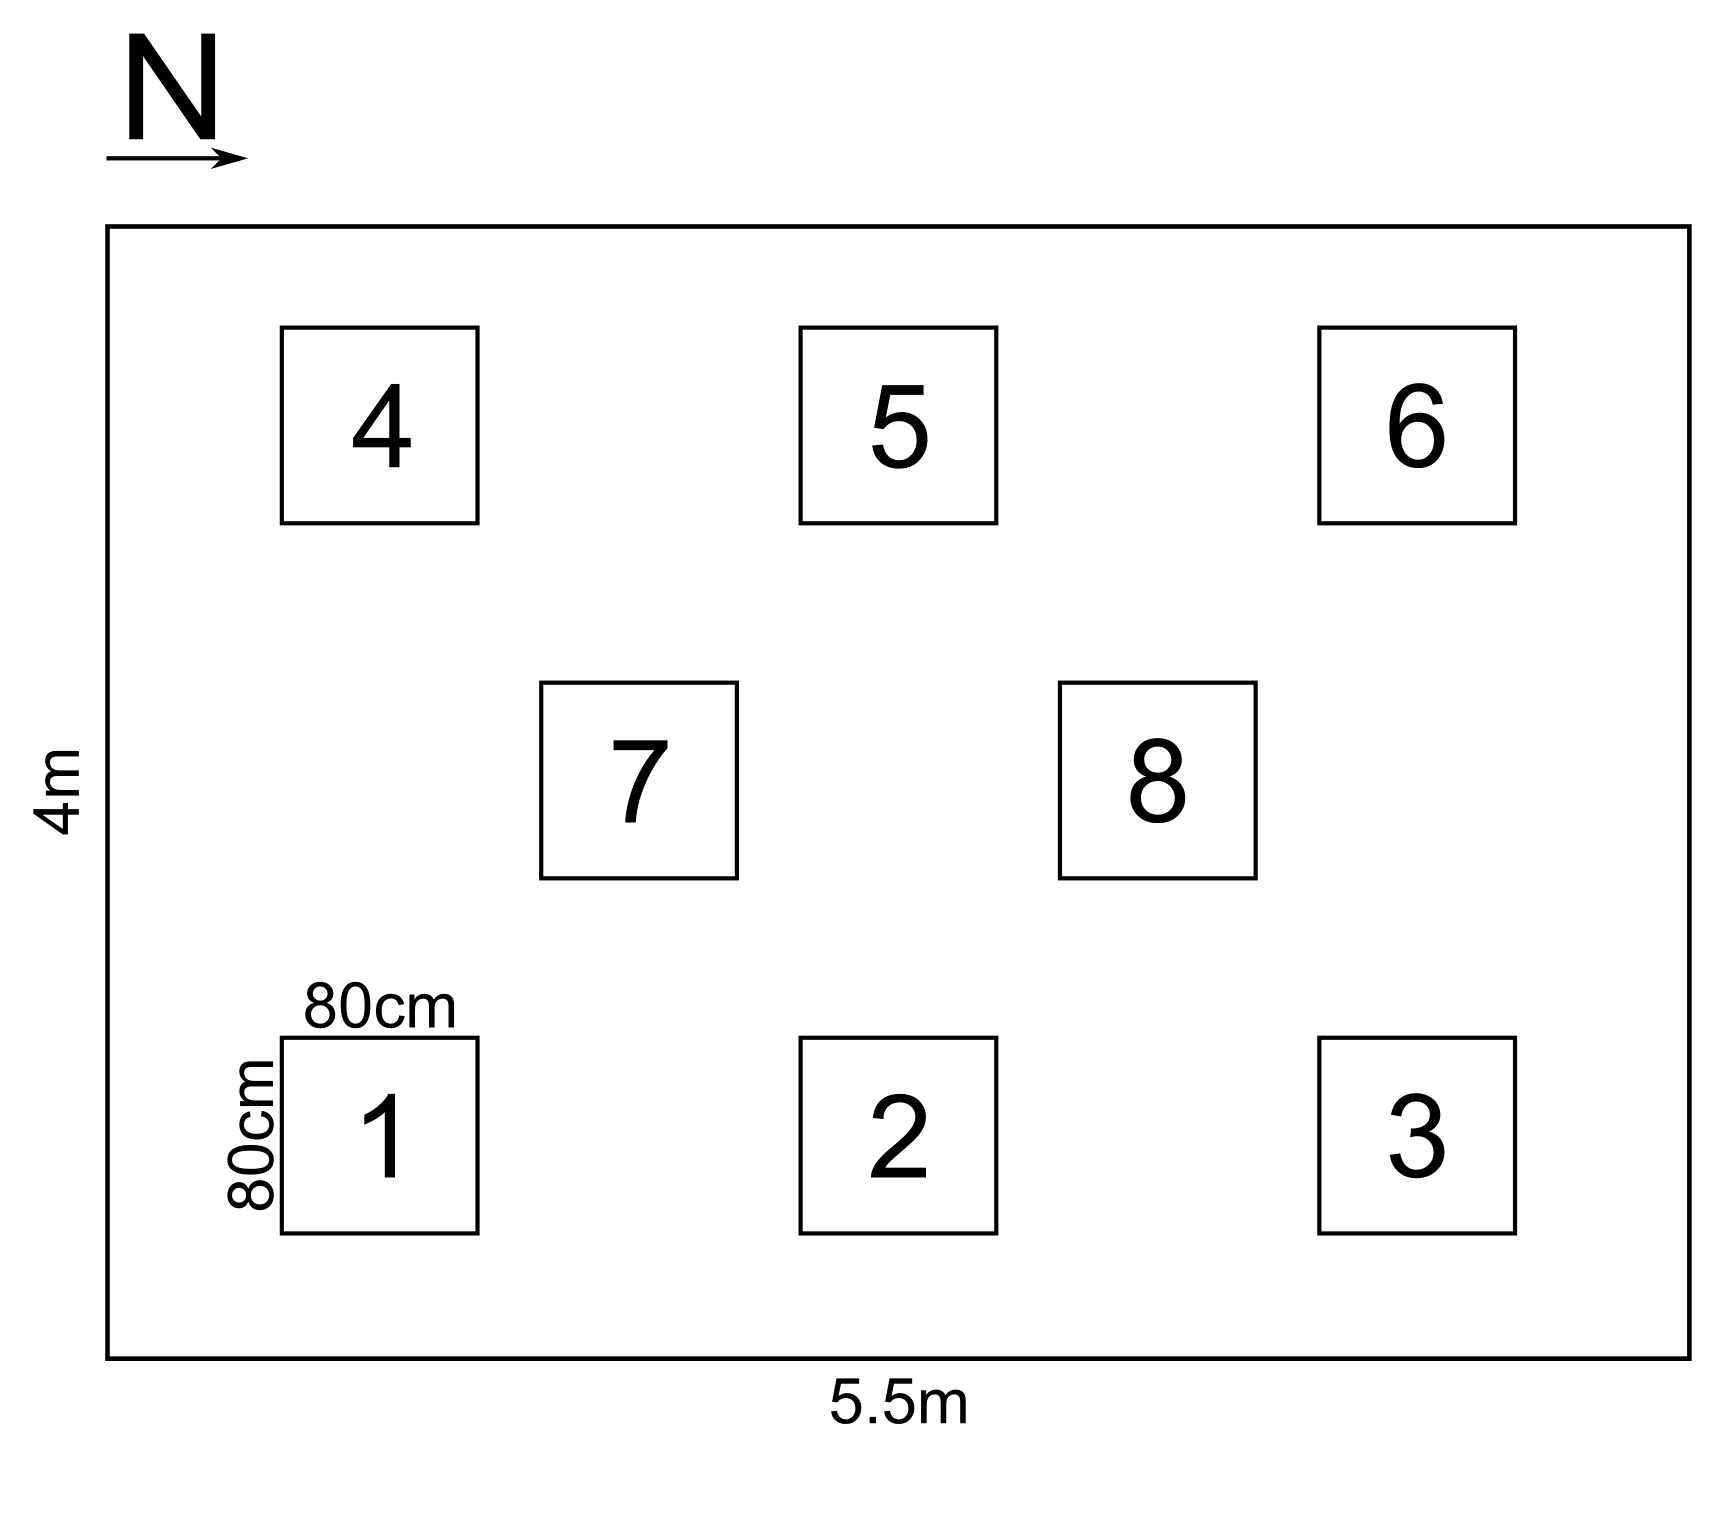
\includegraphics[width=9cm]{Images/plot-design}
 \caption{The distribution of patches within the old invasion plots.}
 \label{fig:plot-design}
\end{figure}


%%%%%%%%%%%%%%%%%%%%%%%%%%
\newpage

\begin{figure} [H] %pairs-plot
\centering
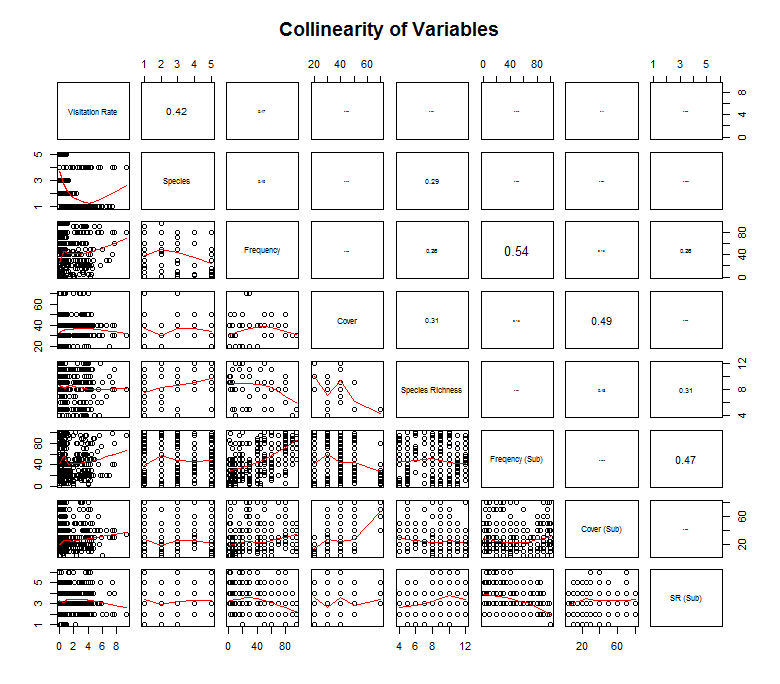
\includegraphics[width=16cm]{Images/pairs-plot}
 \caption{Pairwise correlation of per-flower visitation rate (response variable), species, frequency, floral cover and species richness on plot and patch level. The upper panels contain Pearson correlation coefficients with its size proportional to its value. Parameters correlate on the plot and subplot level but show no strong correlation not among each other.}
 \label{fig:pairs-plot}
\end{figure}

%%%%%%%%%%%%%%%%%%%%%%%%%%

\begin{table}[!htbp] 
  \centering
  \caption{Variance inflation factors (VIF) for the full set of variables. Values are calculated by the "corvif"-function from R-package AED. All values are well below three indicating no collinearity (see \citealt{zuur2007analysing}).}
    \begin{tabular}{ll}
    \toprule
    \textbf{Variable} & \textbf{GVIF}\\
    \midrule
    Visitation Rate  	&  1.26\\
    Species 			 &  1.36\\
    Frequency 	  	    &  1.63\\
    Floral Cover   		 &  1.46\\
    Species Richness     &  1.45\\
    Frequency (Patch) 	    &  1.84\\
    Floral Cover (Patch)		  &  1.37\\
    Species Richness (Patch)    &  1.48\\
    \bottomrule
    \end{tabular}%
\label{tab:VIF}
\end{table}%

%%%%%%%%%%%%%%%%%%%%%%%%%%
\clearpage

\begin{figure} [H] %residuals
\centering
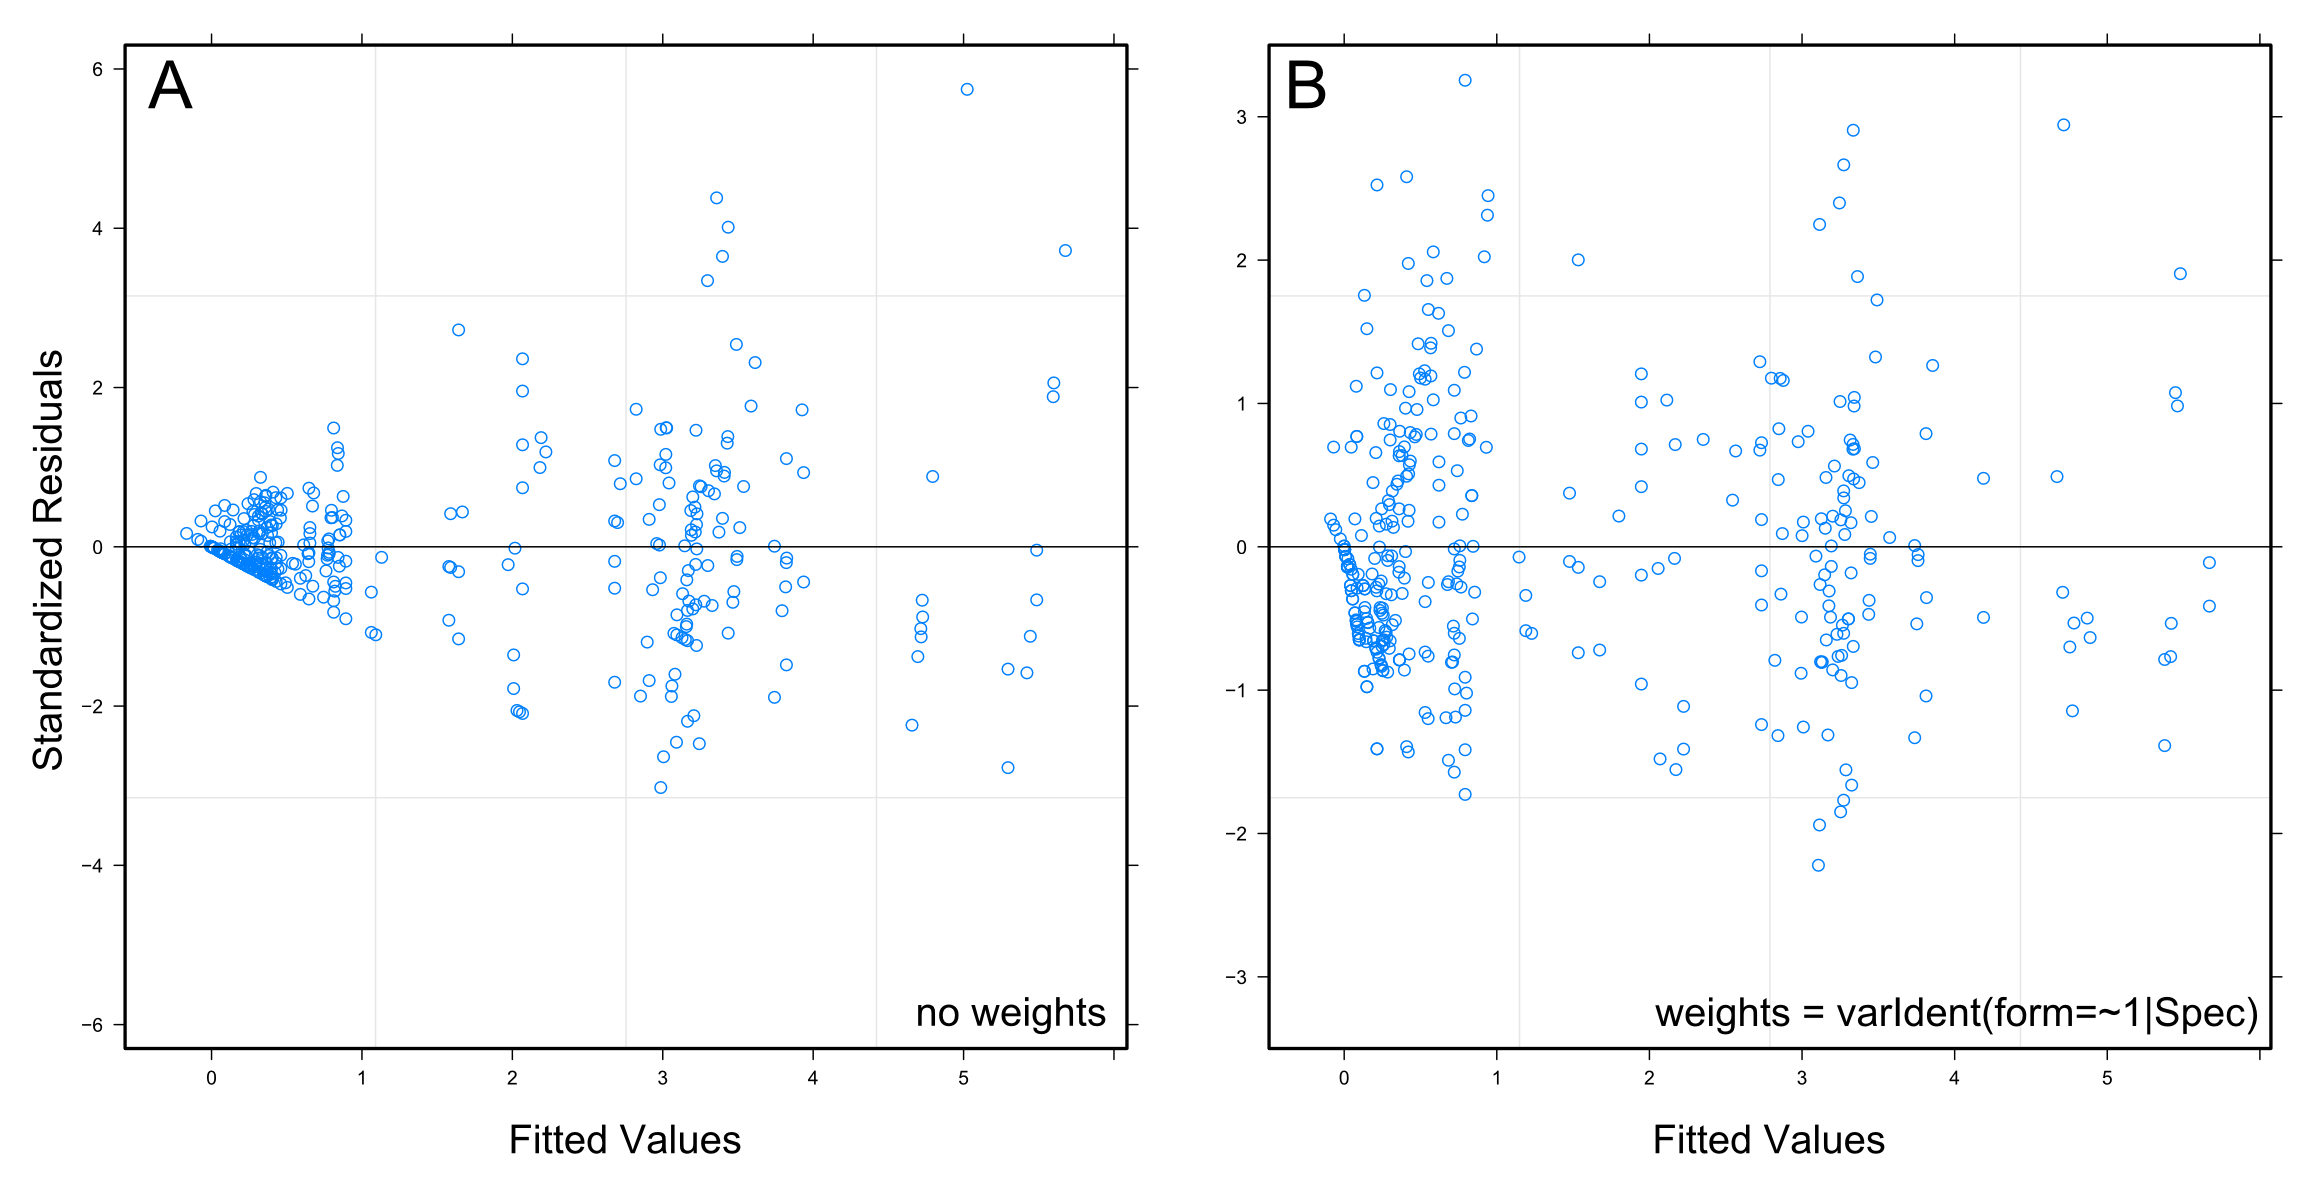
\includegraphics[width=15cm]{Images/residuals}
 \caption{Standardized residuals plotted against fitted values for the final mixed effect model with and without applied weighting. A) Without weighting, the residuals show strong pattern of heteroscedasticity. B) The weighting allows different variance per species. The final model is significantly better with weighting (\textit{L}=393.32, df= 4, \textit{P} $<$ 0.0001)}
 \label{fig:residuals}
\end{figure}

%%%%%%%%%%%%%%%%%%%%%%%%%%

\begin{table} [!htbp]
	\centering
	\caption{Extended output from the linear mixed effect model. Floral cover, species richness and its interactions were removed in the model selection.}
	\begin{tabular}{lccc}
		\toprule
		\textbf{Expanatory Variables} & \textbf{Estimate} & \textbf{$\pm$ SE} &  \textbf{\textit{P}} \\
		\midrule
		Intercept (Ger) & 1.41 & 0.49  & 0.0048 \\ 
		Lat	& -1.58 & 0.58 & 0.0069 \\ 
		Lot	& -1.38 & 0.51 & 0.0075 \\ 
		Ono	& -1.31 & 1.06 & 0.2182 \\ 
		TP	& -1.39 & 0.5  & 0.0060 \\ 
		\addlinespace[0.2cm]
		Frequency	& 0.11 & 0.05 & 0.0147 \\
		Frequency$^{2}$	& -0.002 &  $<$ 0.01 & 0.0699 \\ 
		Frequency$^{3}$	& $<$ 0.01 & $<$ 0.01 & 0.1174 \\ 
		\addlinespace[0.2cm]
		Frequency x Lat	& -0.09 & 0.05 & 0.0925 \\
		Frequency x Lot	& -0.09 &  0.05 & 0.0687 \\ 
		Frequency x Ono	& 0.32 & 0.14 & 0.0183 \\ 
		Frequency x TP	& -0.1 & 0.05 & 0.0425 \\
		\addlinespace[0.2cm] 
		Frequency$^{2}$ x Lat	& $<$ 0.01 & $<$ 0.01 & 0.1013 \\
		Frequency$^{2}$ x Lot	& $<$ 0.01 & $<$ 0.01 & 0.2053 \\ 
		Frequency$^{2}$ x Ono	& -0.01 & $<$ 0.01 & 0.0113 \\ 
		Frequency$^{2}$ x TP	& $<$ 0.01 & $<$ 0.01 & 0.1479 \\ 
		\addlinespace[0.2cm]
		Frequency$^{3}$ x Lat	& $>$ -0.01 & $<$ 0.01 & 0.0966 \\
		Frequency$^{3}$ x Lot	& $>$ -0.01 & $<$ 0.01 & 0.2996 \\ 
		Frequency$^{3}$ x Ono	& $<$ 0.01 & $<$ 0.01 & 0.0086 \\ 
		Frequency$^{3}$ x TP	& $>$ -0.01 & $<$ 0.01 & 0.2283 \\
		\bottomrule
	\end{tabular}
	\label{tab:summary} 
\end{table}

\clearpage
\newgeometry{margin=1cm}
\thispagestyle{empty}

\begin{sidewaystable}[!h] %Parameter Values
	\footnotesize
	\centering
	\caption{The full set of parameters and default values used in the model. }
	\begin{tabular}{l l l l l l}
		\toprule
		\textbf{Parameter} & \textbf{Description} & \textbf{NetLogo-Type} & 		  \textbf{Type} & \textbf{Value} & \textbf{Reference} \\
		\midrule
		\addlinespace[0.2cm]
		\multicolumn{6}{l}{\textsc{Setup Parameters:}} \\ 
		\addlinespace[0.2cm]
		
		area  & "world" in NetLogo, defined by a grid of cells called patches &       & integer & 100x100 &  \\
		
		patch-size & Size of one grid-cell in NetLogo. Can be either a flower or grass &       & float & 0.1m² &  \\
		
		tick  & One time-unit in NetLogo &       & integer & 1s    &  \\
		
		flower-cover & Proportion of grid cells containing a flower & global & integer &       5, 10, 20, 30, 50 &  \\
		
		frequency & Proportion of flowers which are species A 	($Freq_{B} = 100 - Freq_{A}$)  & global & integer &   0-100\%    &  \\
		
		cluster-number & Average number of flowers per cluster & global & integer &  1, 2, 5, 10, 20, 50, 75, 100 &  \\
		
		number-bees & Initial number of pollinators in the model & global & integer &  10    & 0.0004 - 1 bee/m² \citep{essenberg2012explaining} \\
		
		\addlinespace[0.2cm]
		\multicolumn{ 6 } {l} {\textsc{Behavioural Parameters:}} \\ 
		
		search-speed & Distance a pollinator can move per time step & bees-own & integer & 0.1m /sec  & \begin{tabular}{@{}l@{}} \citealt{kunin1991few} in \citealt{kunin1996pollinator}  \\  0.09-0.17 \citep{essenberg2012explaining} \end{tabular} \\
		
		stdev-angle & Standard deviation for the normal distribution used in the CRW & global & integer &  30    & \citealt{waddington1980flight}  \\
		
		flightsteps-until-change & Seconds of unsuccessful search before the preference changes & bees-own & integer & 5s ( = 5 ticks) &  \citealt{chittka1997foraging,kunin1993sex}  \\
		
		length-memory & How many flowers can a bee remember to avoid double-visiting  & bees-own & integer & 4     & \citealt{goulson2000pollinators}, see \citealt{goulson1999foraging} for review \\
		
		view  & Value for the radius of grid-cells a pollinator can see (cone-view of 180°) & bees-own & integer & 0.7m ( = 6 grid-cells) &  \begin{tabular}{@{}l@{}} \citealt{dyer2008comparative, wertlen2008detection} \\ \citealt{ne2001effect} \end{tabular} \\
		
		array & \begin{tabular}{@{}l@{}} Array of all suitable flowers (referred, non-visited)\\ in sight of the pollinator \end{tabular} & bees-own & Array &       &  \\
		
		reward-function & How much reward is replenished per second & flowers-own & float & 0.00004 J/s   &  \\
		
		handling-time & The time a pollinator needs for exploiting the floral reward & bees-own & integer & reward * 4s + 0.5s (+ 3s) & \citealt{roubik1992ecology} in \citealt{kunin1996pollinator} \\
		
		reward & \begin{tabular}{@{}l@{}}Reward in Joule the flower has to offer. \\  Exploited with each visit, replenished over time \end{tabular} & flowers-own   & float & reward(max) = 1J & \citealt{kunin1991few} in \citealt{kunin1996pollinator}  \\
		
		pollen carry-over rate & \begin{tabular}{@{}l@{}} Number of heterospecific visits within \\ a successful pollination is possible \end{tabular} & flowers-own & integer & 1, 2, 4, 6, 8, 16  & \citealt{benadi2012population} \\
		
		flower-memory & A list of flower-locations  & bees-own & string &    4   & see \citealt{goulson1999foraging} for review \\
		
		reward-memory & A list of the last gained rewards & bees-own & string &    4   &  \\
		
		change-prob & \begin{tabular}{@{}l@{}}Probability to change the preferred flower type. \\ Increases with low reward and long search times \end{tabular} & bees-own & float &       &  \\
		
		choice & Current flower choice for the pollinator (for constancy) & bees-own & boolean &       &  \\
		
		\bottomrule
	\end{tabular}%
	\label{tab:parametervalues}%
\end{sidewaystable}%
\restoregeometry

%%%%%%%%%%%%%%%%%%%%%%%%%%%%%%%%%%%%%%%%%%%%%%%%%%%%%%%%%%
\newpage
\clearpage

\begin{figure} [!h]
	\centering
	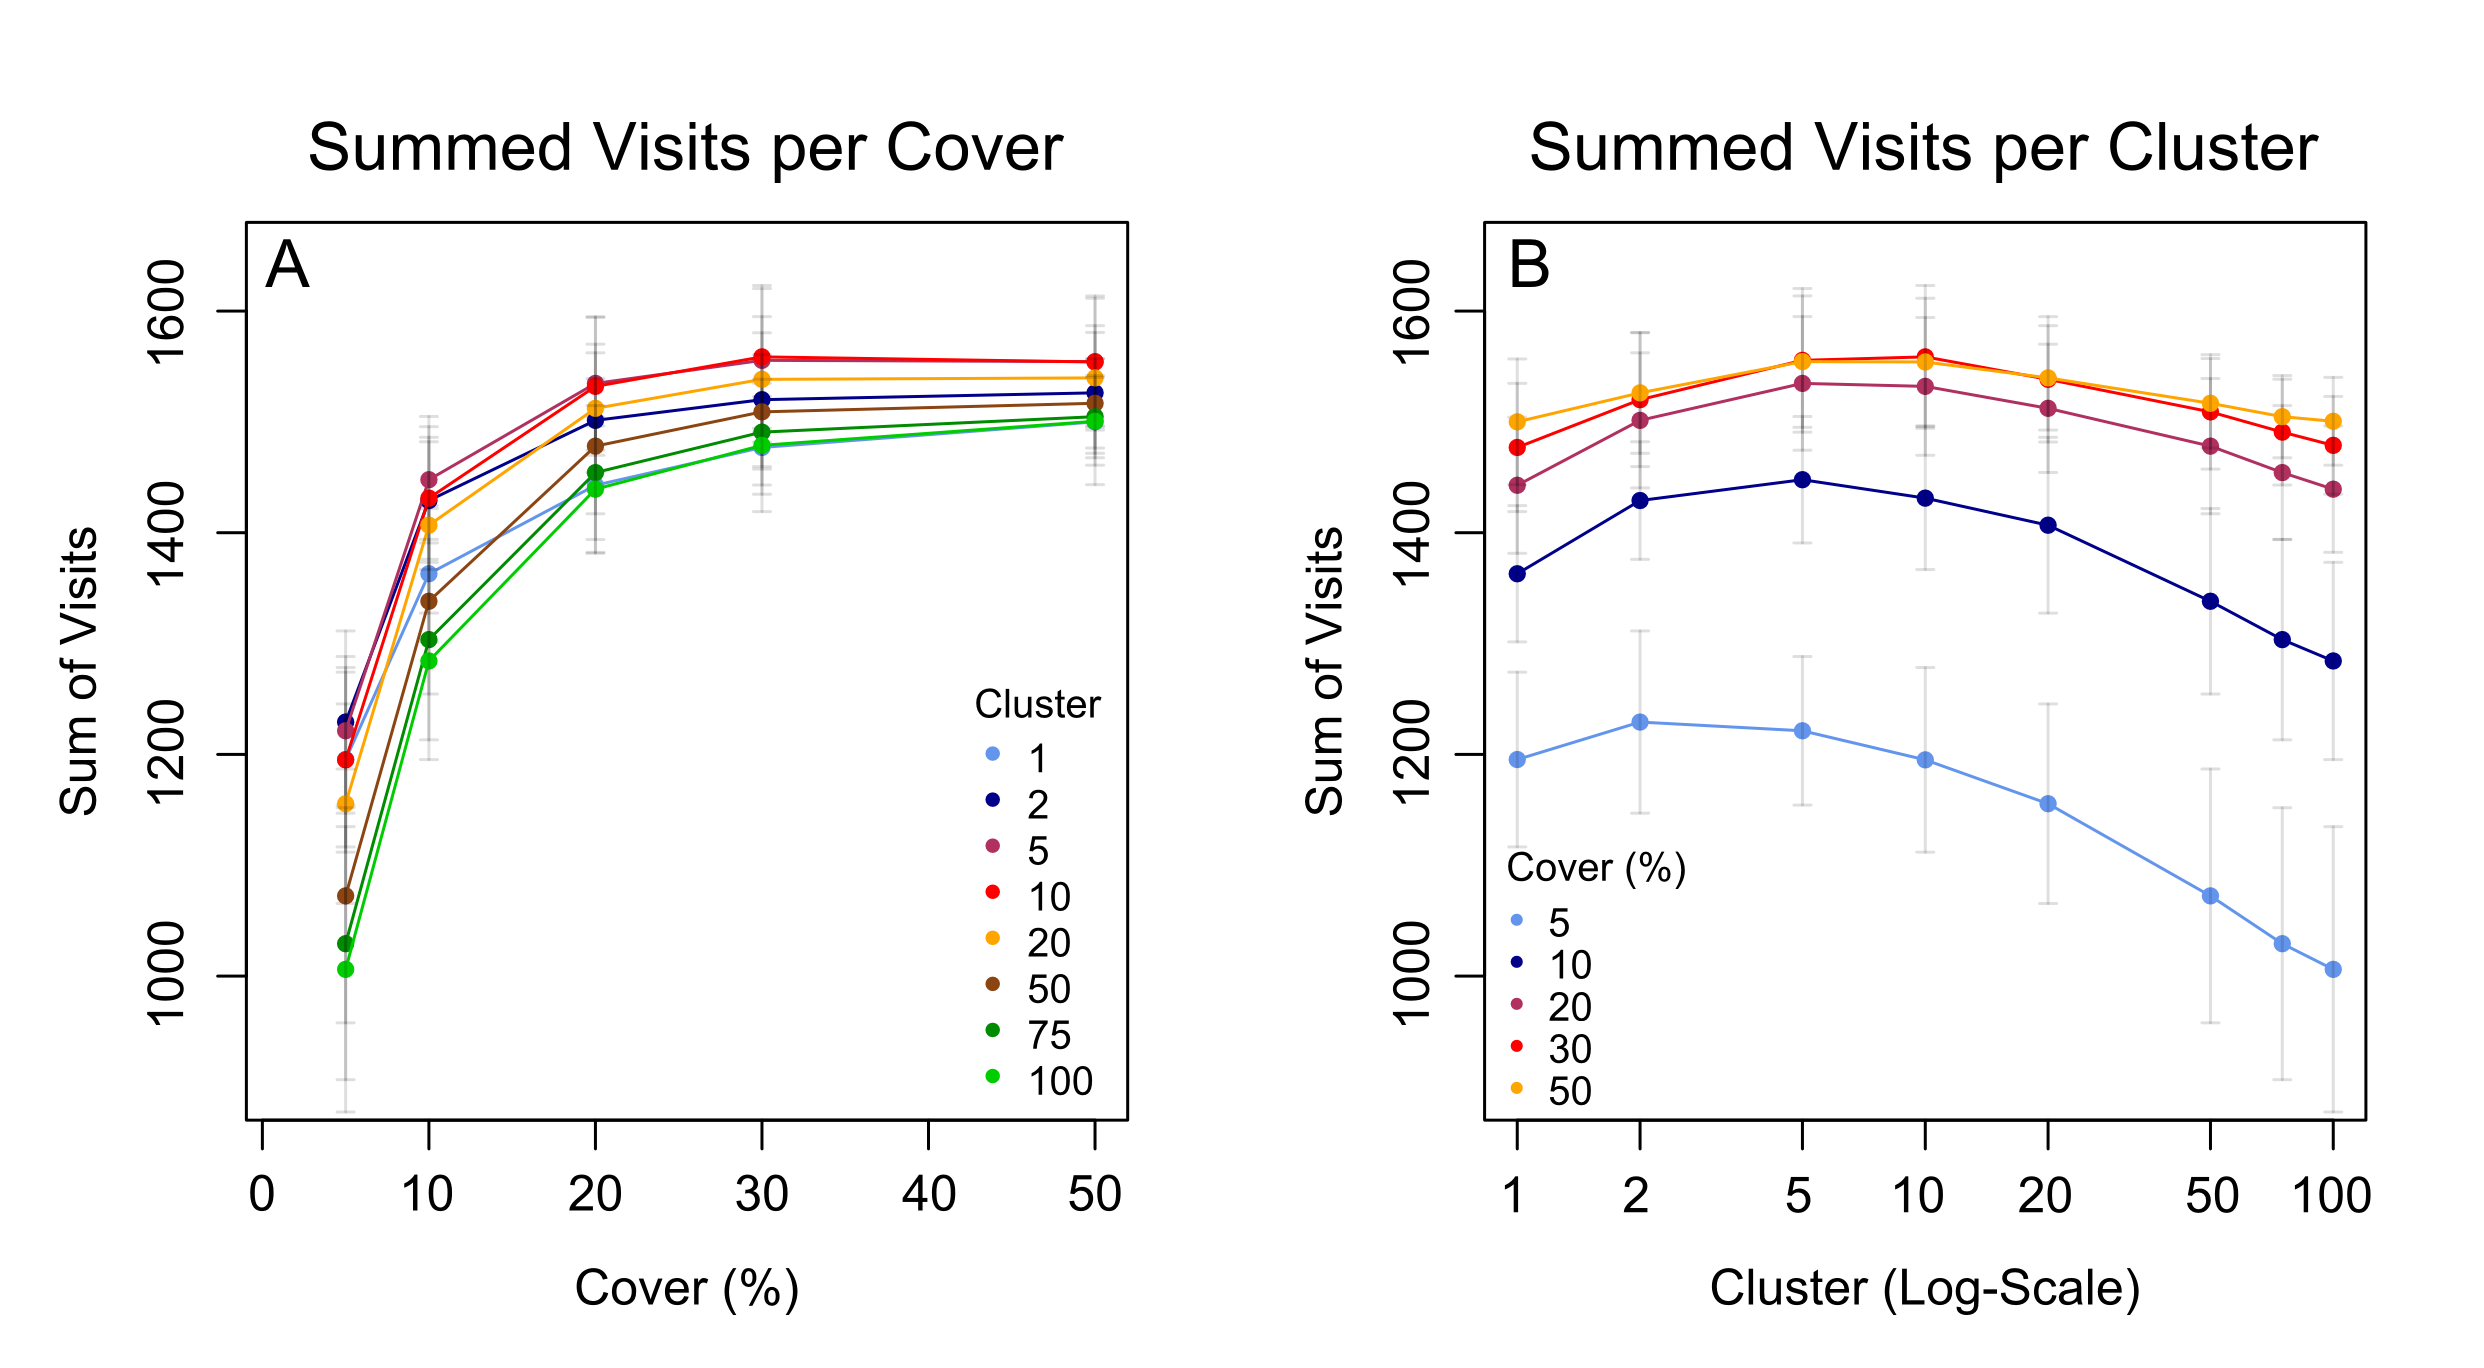
\includegraphics[width=14cm]{Images/nonfreq}
	\caption{Frequency independent influence of floral cover and cluster size on the sum of all visits to both species together. A) Cover strongly influences the number of visits as it reduces the flight and search time and shows a saturated relationship for all cluster values. This matches the Holling's type II functional response. B) The degree of clustering influences the sum of visits in a hump-shaped function. The maximum lays between 5 and 10 flowers per cluster  (depending on the cover). A small aggregation of flowers reduces search times but keeps the next patch within visible distance. The bigger the cluster, the more difficult for the bee-agent to find the next one.}
	\label{fig:nonfreq}
\end{figure}

\clearpage

\begin{figure} [h!]
	\centering
	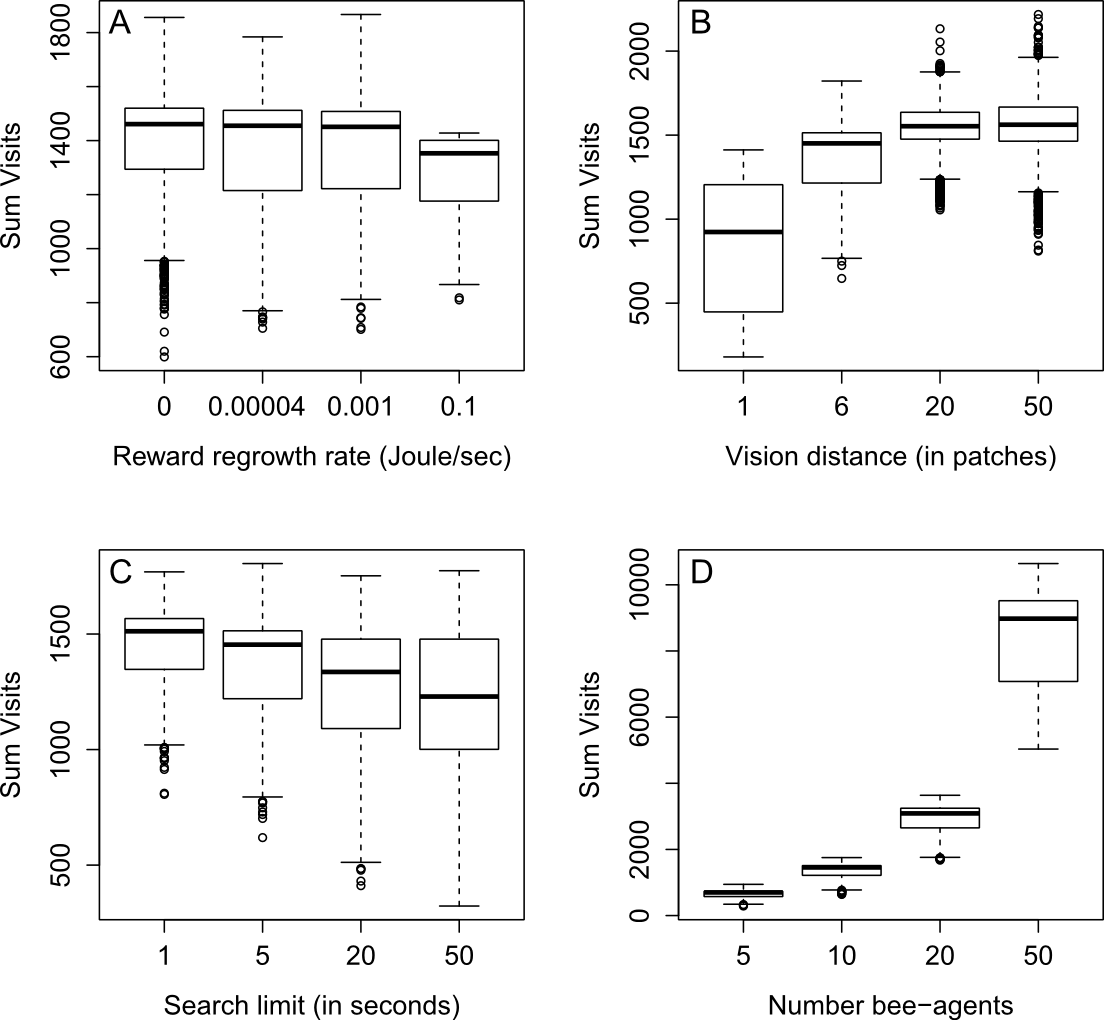
\includegraphics[width=14cm]{Images/SA_SUM}
	\caption{The influence of reward replenishment, vision, search limit and number of bee-agents on the sum of visits within a 1000 time-step simulation run. A) An unnatural high reward replenishment rate (if the flowers are refilled within 10 time steps) has a small negative influence on the visits.  B) Bee-agents with a far field of view can detect flowers faster, move in a direct way towards them and be therefore more efficient. However, the curve is saturated at a view of 20 patches. C) An increase in search time limit decreases the sum of visits and spread the variance. Bees-agents will keep searching for rare flowers instead of switching to the common species. D) As assumed, more bees lead to more visits.} 
	\label{fig:SA_SUM}
\end{figure}

\clearpage

\begin{figure} [!h] %
	\centering
	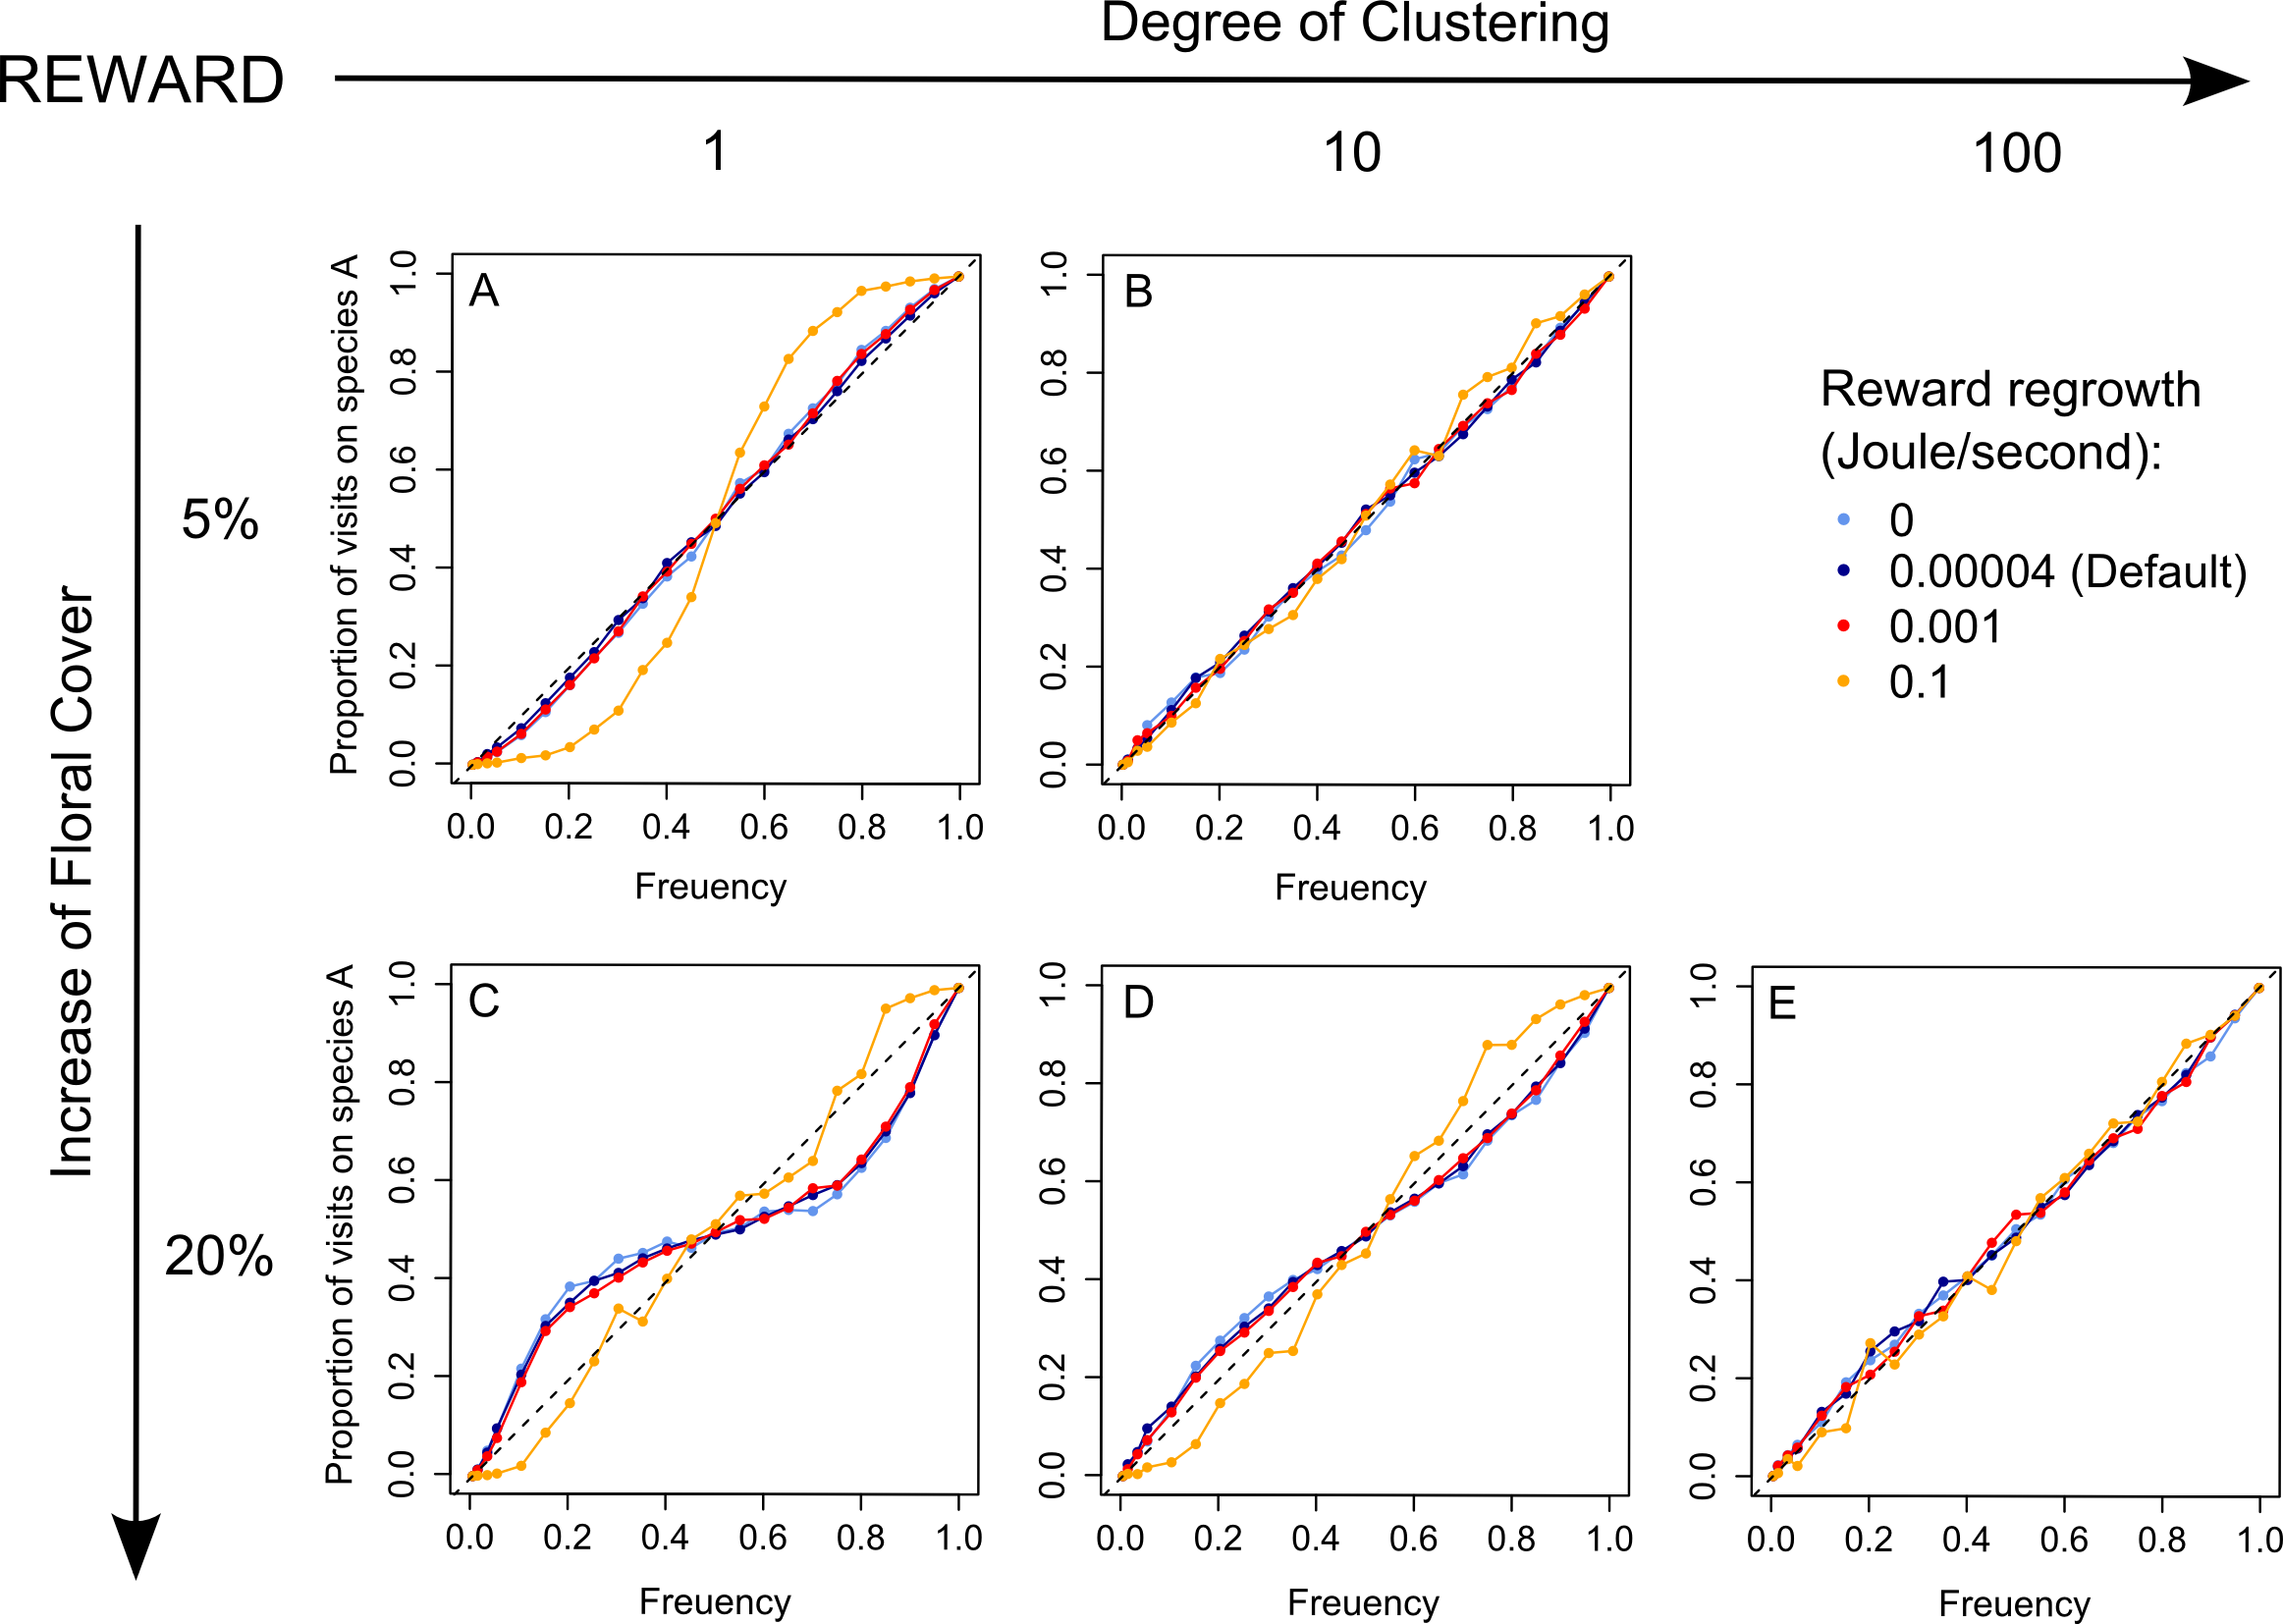
\includegraphics[width=14cm]{Images/SA_reward}
	\caption{Outcome of the model if the reward replenishment function is changed to 0, 0.004, 0.001 and 0.1 Joules per time step. Only the unnatural high reward function (complete regrowth after 10 seconds) has an influence on the frequency dependence: The bee-agents have no more reason to change preference due to bad reward. This favors the more common species as shown in the opposite curving for no-cluster environments. A lower replenishment rate has no effect.} 
	\label{fig:SA_reward}
\end{figure}

\clearpage


\begin{figure} [!h]
	\centering
	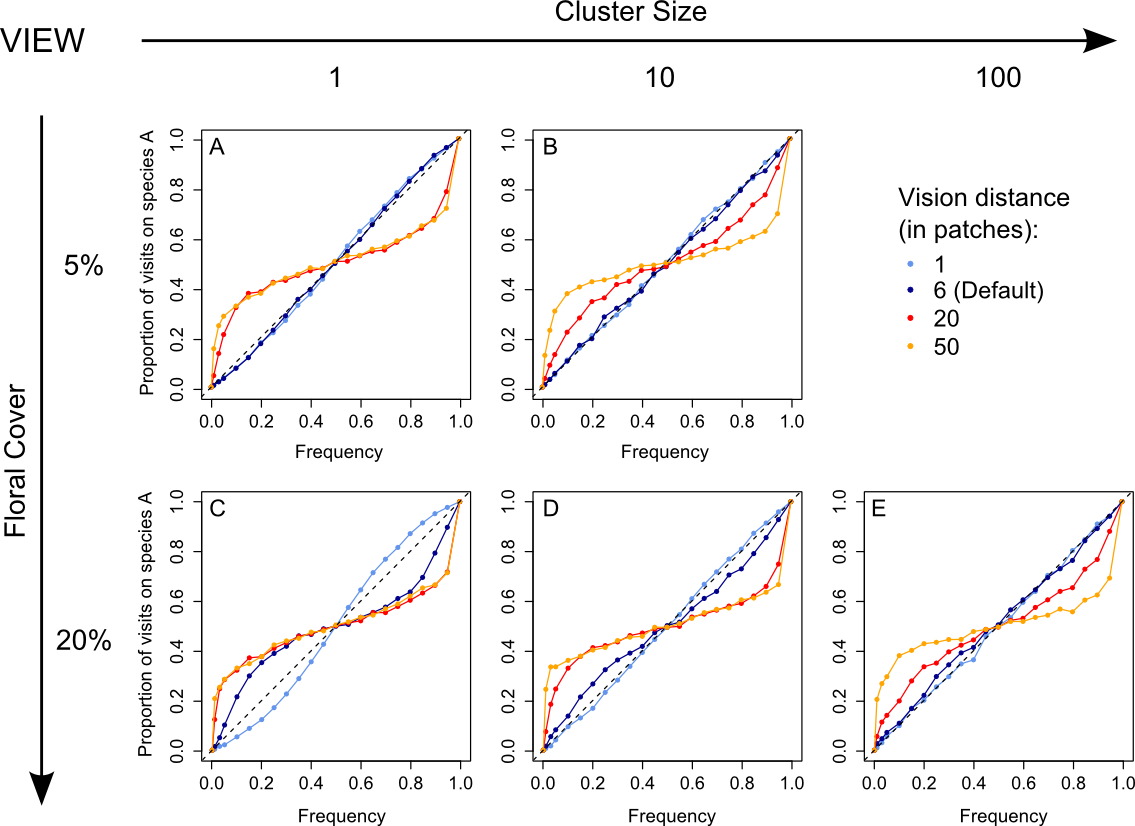
\includegraphics[width=14cm]{Images/SA_view}
	\caption{Effect of increased or reduced vision for the bee-agent. The vision influences the behavior of the bee-agent. If it sees far, it can move on direct way towards the next preferred flower and saves searching time. But it also flies longer distances instead of changing to the common species. A large vision therefore increases the frequency dependence and a very low vision shifts the advantage towards the more abundant species.}
	\label{fig:SA_view}
\end{figure}

\clearpage


\begin{figure} [!h] 
	\centering
	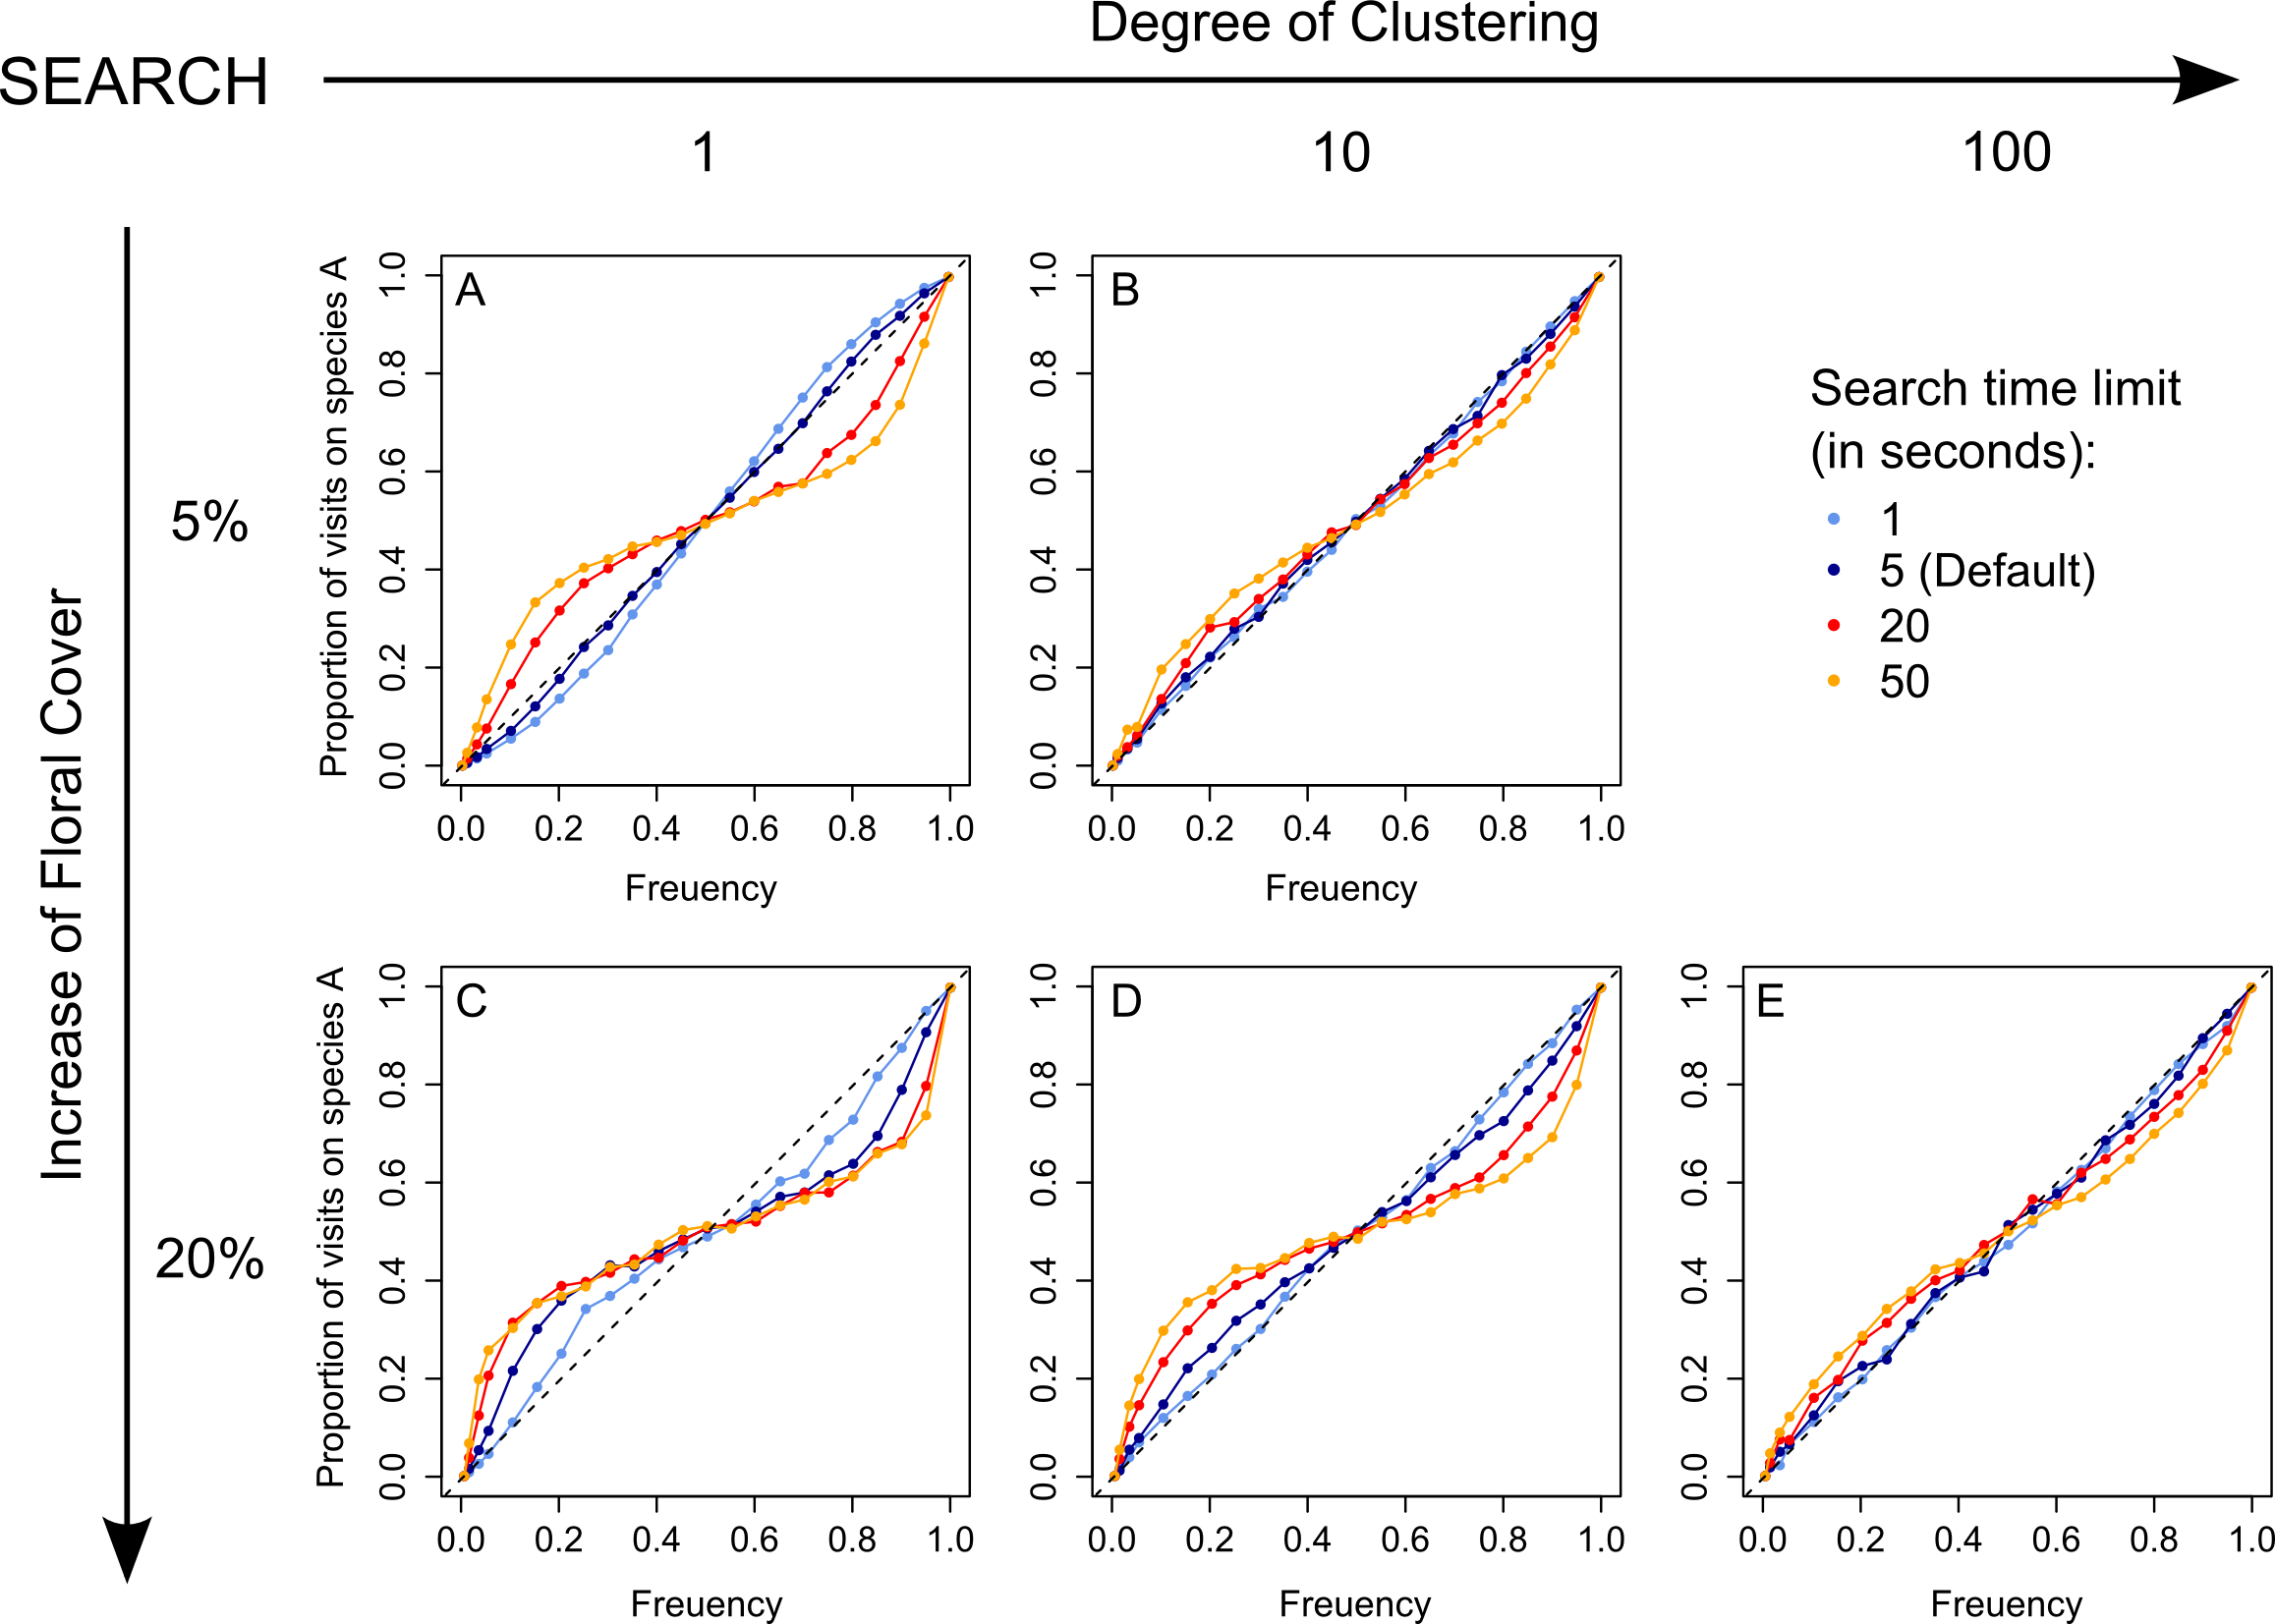
\includegraphics[width=14cm]{Images/SA_flight}
	\caption{Sensitivity analysis for search limits of 1,5, 20 and 50 seconds. The search limit is the number of seconds within a bee-agent searches for a unvisited and preferred flower, moving around the meadow by a correlated random walk. After the search limit is reached, the probability to change its flower preference increases with every additional second of unsuccessful search by 10\%. The search limit has a similar effect on the outcome of the model as the vision because it also influences the change probability. With a higher search time, the bee-agent continues searing instead of switching to the more abundant flower, the frequency dependence is increased. A higher cluster value weakens the effect.}
	\label{fig:SA_flight}
\end{figure}

\clearpage

\begin{figure} [!h]
	\centering
	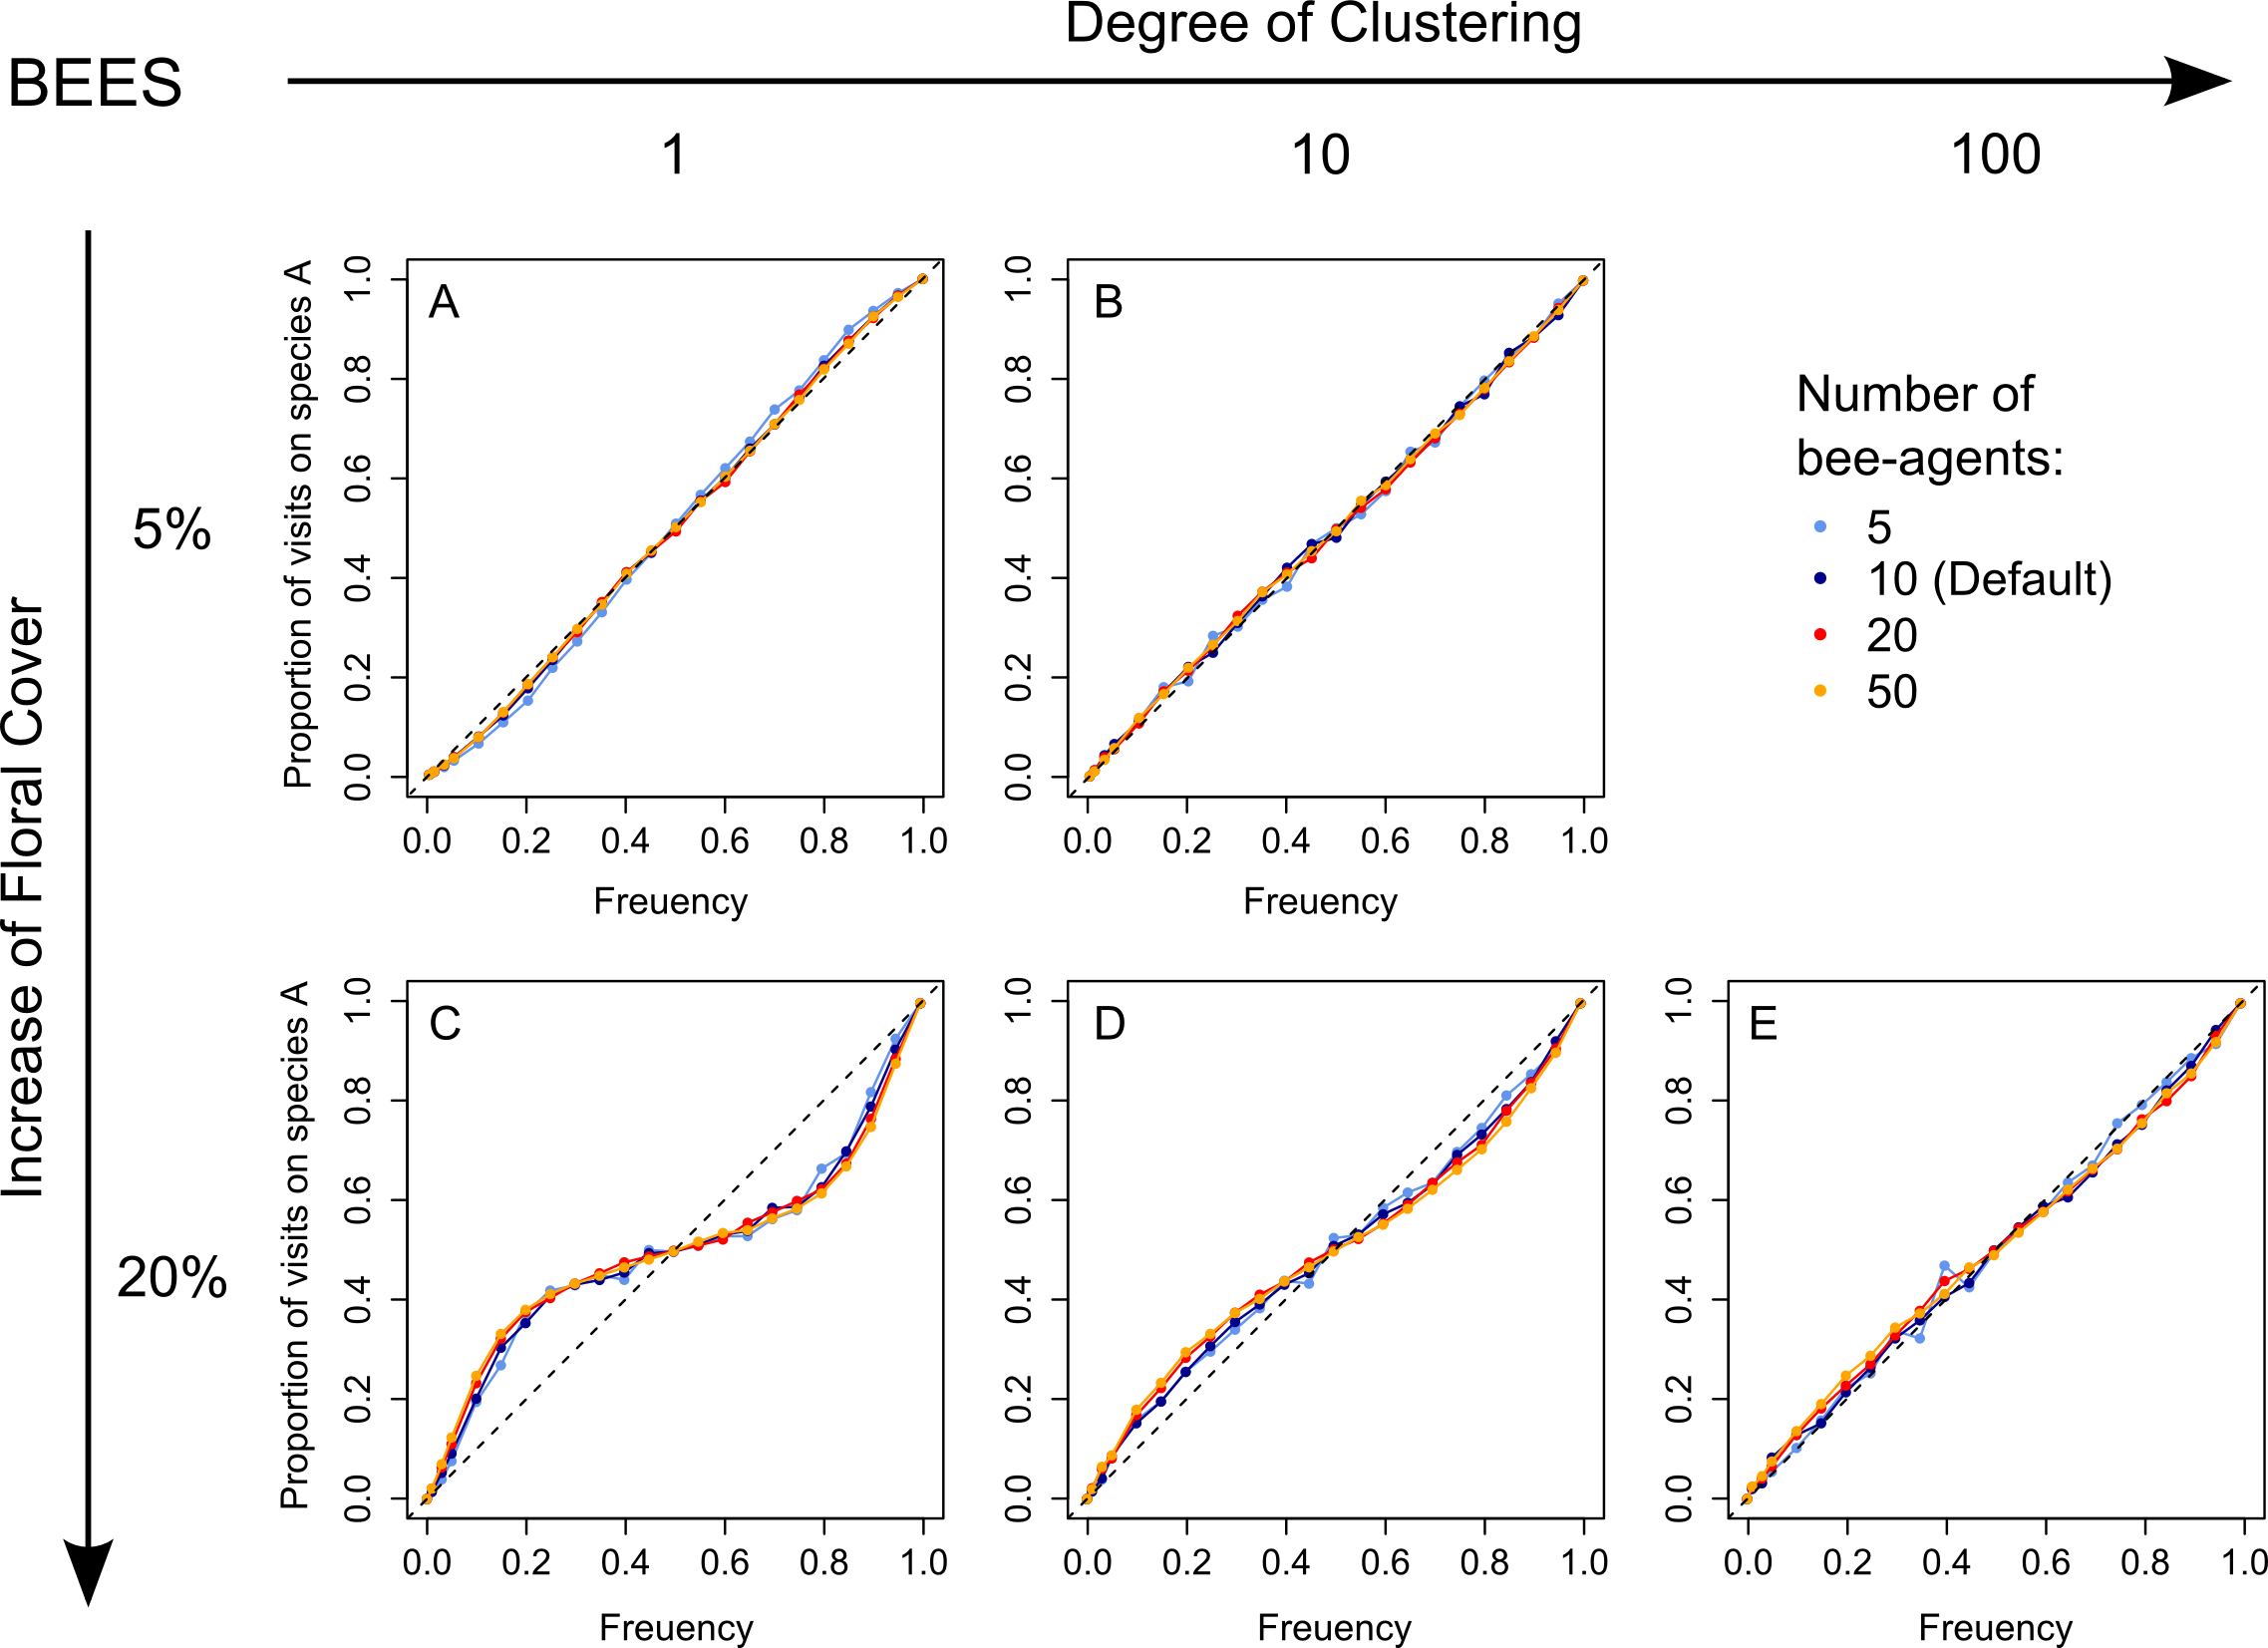
\includegraphics[width=14cm]{Images/SA_bees}
	\caption{Results of the model for 5, 10, 20 and 50 bee-agents on the meadow. The proportion of visits does not change, only the absolute numbers. Therefore has the pollinator density no influence on the frequency dependence.}
	\label{fig:SA_bees}
\end{figure}


\begin{figure} [!h]
	\centering
	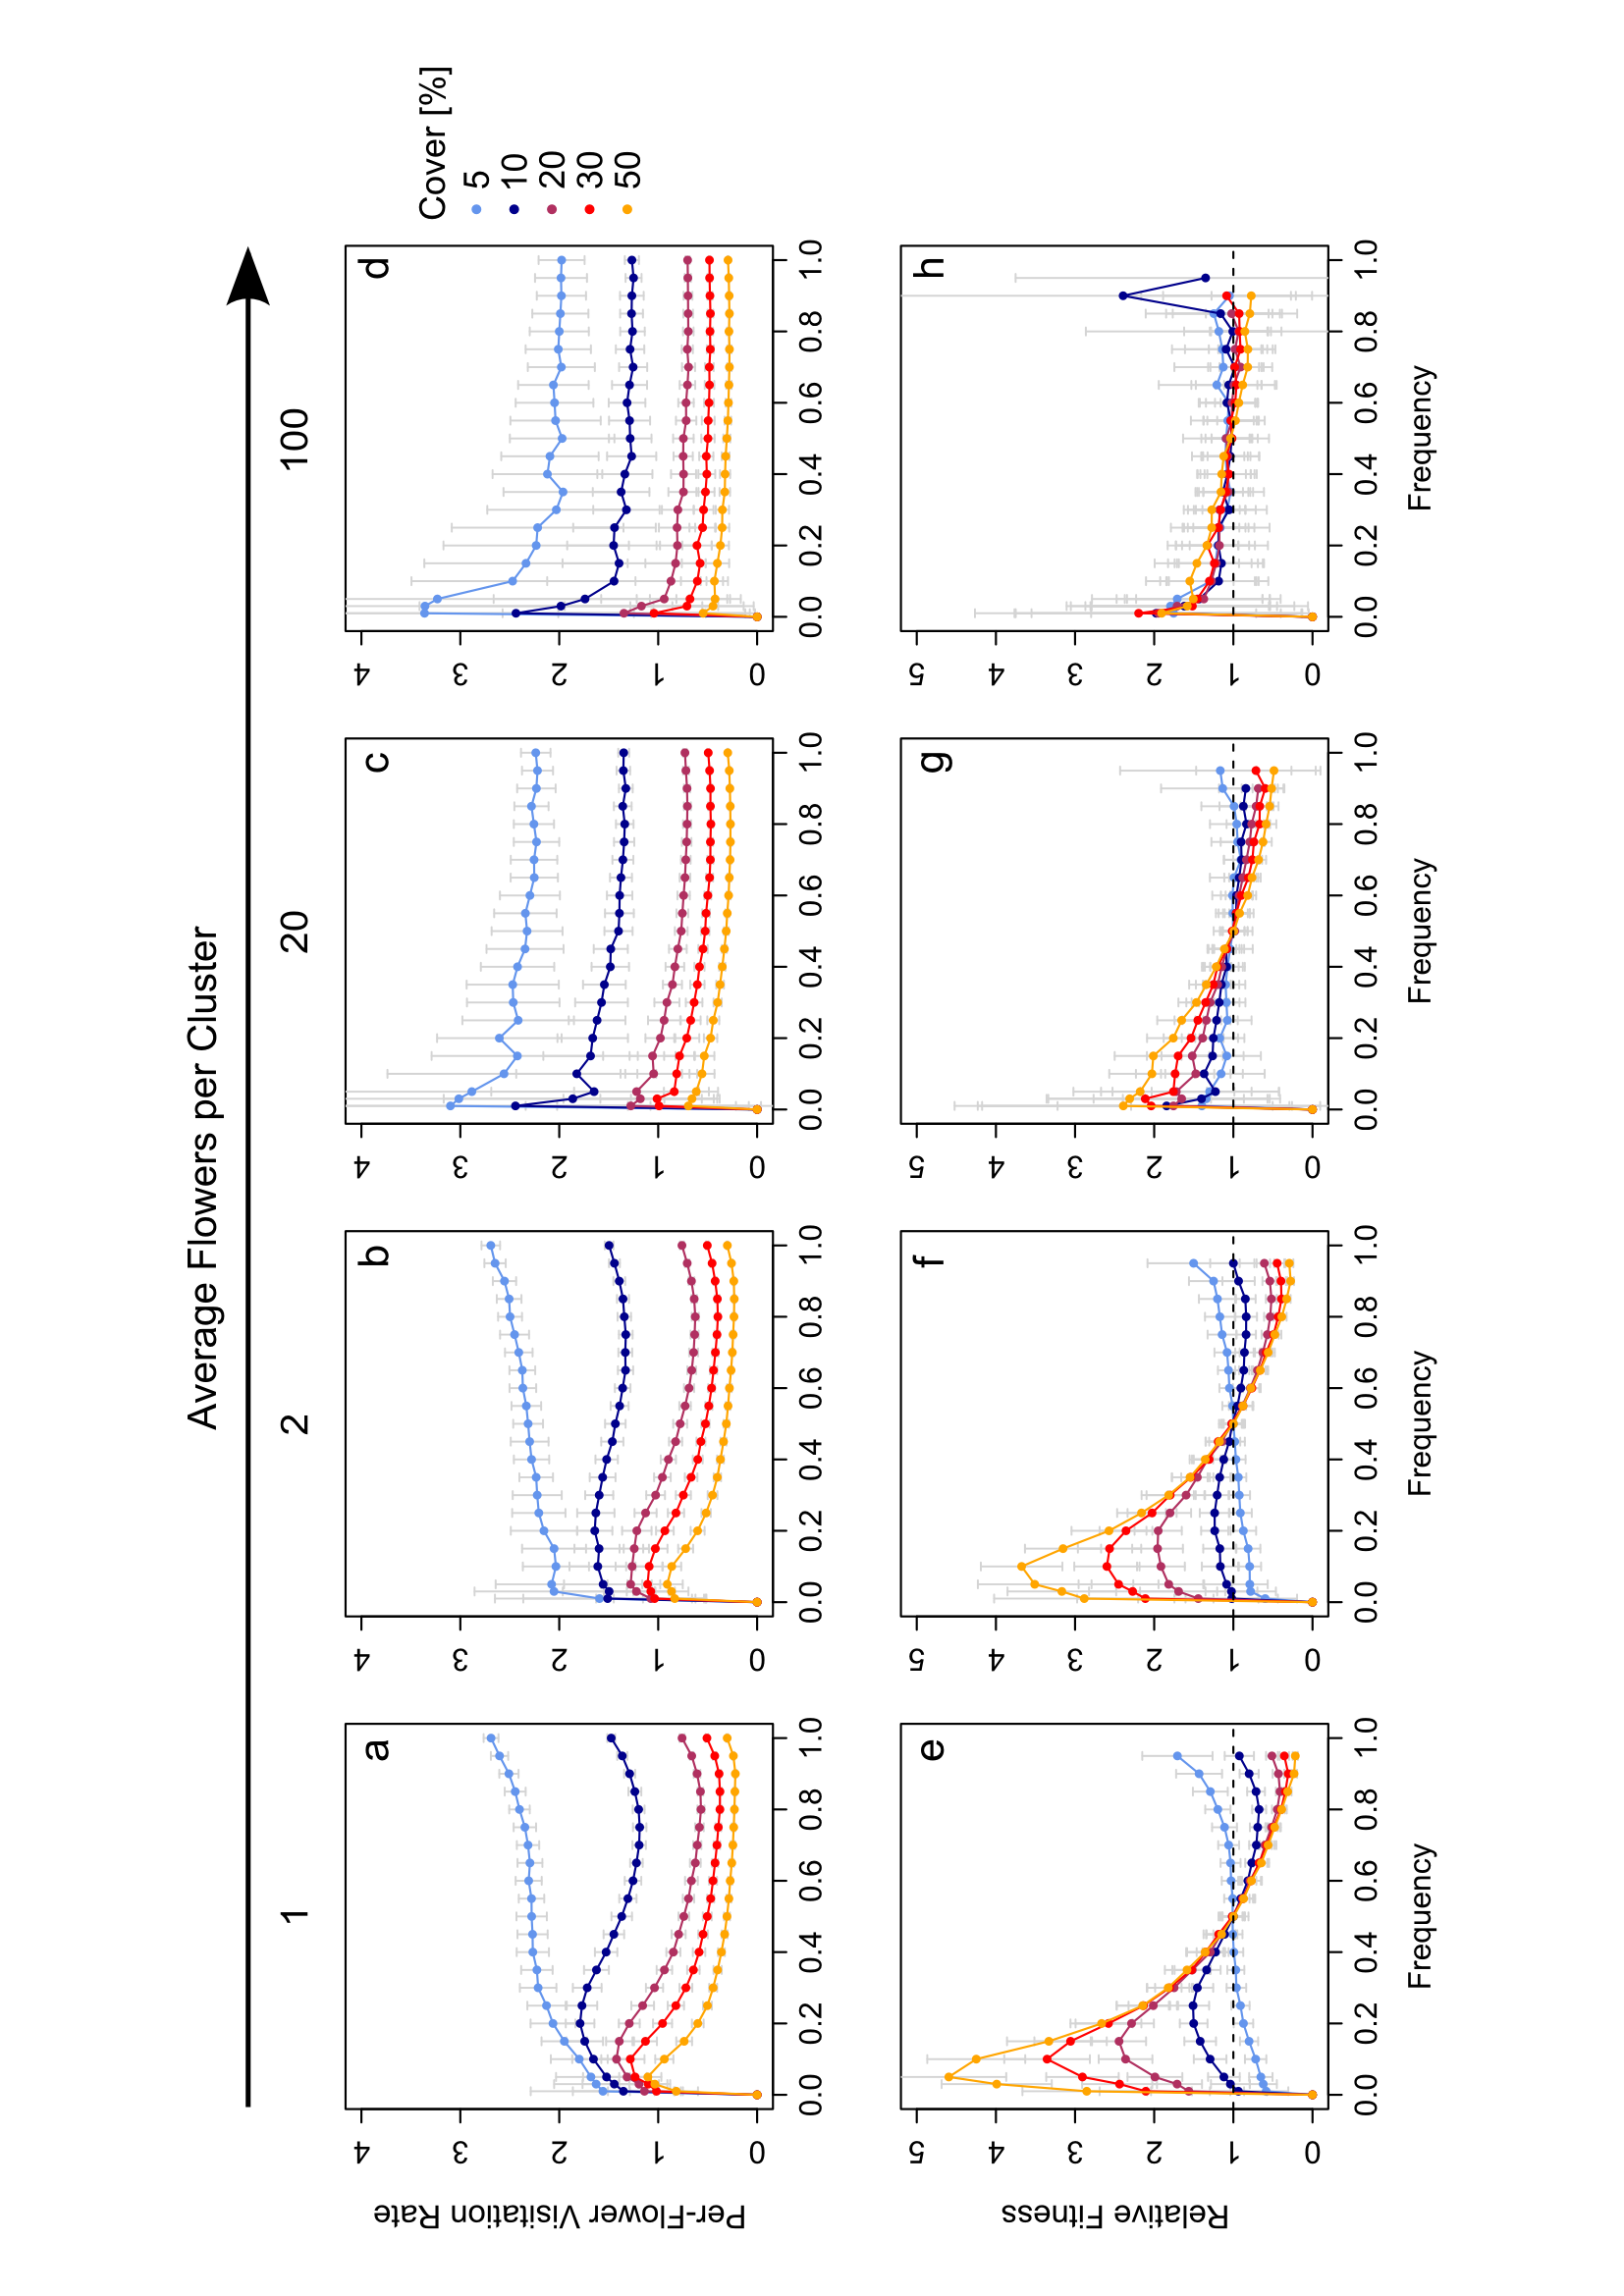
\includegraphics[width=15cm]{Images/PFVgross}
	\caption{Enlarged version of Figure ~\ref{fig:PFV}. The per-flower visitation rate shows a frequency dependence with a cubic relationship. The same data is plotted relative to per-flower visitation of the other species to visualize the relative fitness and intensity of frequency dependence (e-h).}
	\label{fig:PFVgross}
\end{figure}

\begin{figure} [!h]
	\centering
	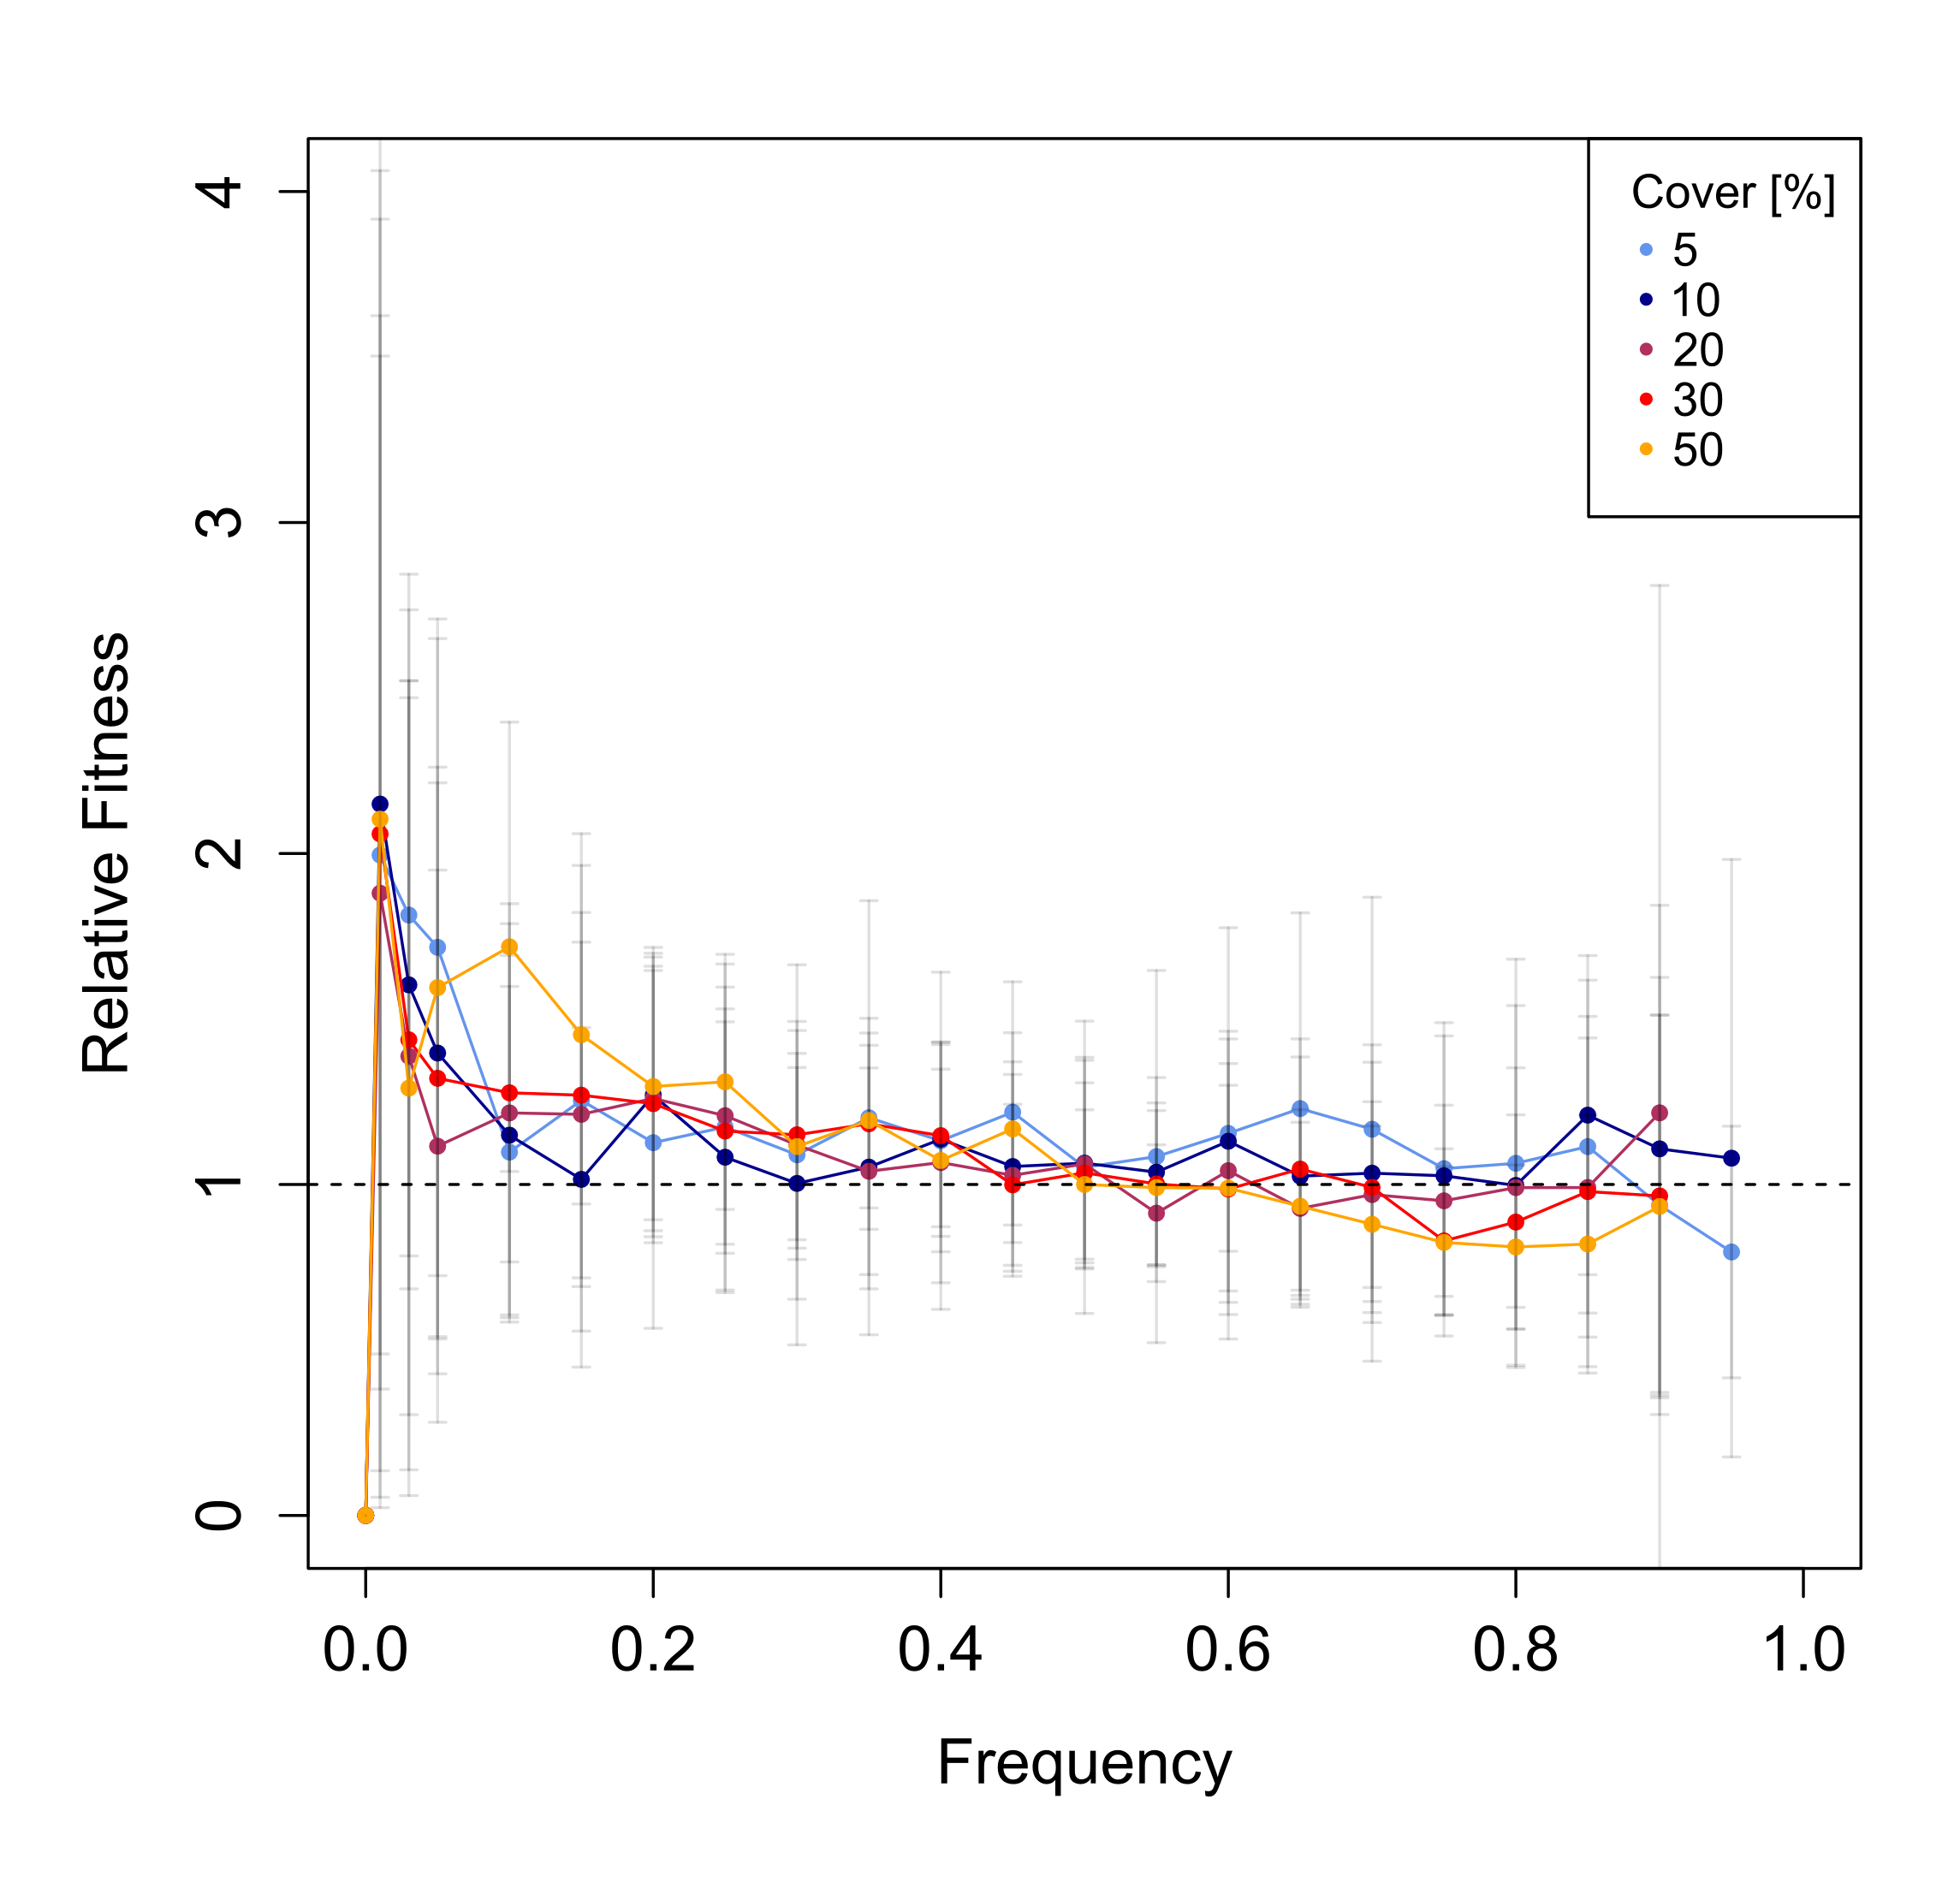
\includegraphics[width=10cm]{Images/Outlier}
	\caption{Results of the model for an average of 100 flowers per cluster. The per-flower visitation of species A was divided through the per-flower visitation of species B to observe the relative fitness. Due to a statistical outlier in the main analysis (Fig.~\ref{fig:PFV}h), the model was run again with 50 runs per parameter combination. Points are the mean of all runs with grey error bars.}
	\label{fig:outlier}
\end{figure}

%%%%%%%%%%%%%%%%%%%%%%%%%%%%%%%%%%%%%%%%%%%%%%%%%%%%%%%%%%%%%%%%%%%%%%%%

